\documentclass[twoside]{book}

% Packages required by doxygen
\usepackage{fixltx2e}
\usepackage{calc}
\usepackage{doxygen}
\usepackage[export]{adjustbox} % also loads graphicx
\usepackage{graphicx}
\usepackage[utf8]{inputenc}
\usepackage{makeidx}
\usepackage{multicol}
\usepackage{multirow}
\PassOptionsToPackage{warn}{textcomp}
\usepackage{textcomp}
\usepackage[nointegrals]{wasysym}
\usepackage[table]{xcolor}

% Font selection
\usepackage[T1]{fontenc}
\usepackage[scaled=.90]{helvet}
\usepackage{courier}
\usepackage{amssymb}
\usepackage{sectsty}
\renewcommand{\familydefault}{\sfdefault}
\allsectionsfont{%
  \fontseries{bc}\selectfont%
  \color{darkgray}%
}
\renewcommand{\DoxyLabelFont}{%
  \fontseries{bc}\selectfont%
  \color{darkgray}%
}
\newcommand{\+}{\discretionary{\mbox{\scriptsize$\hookleftarrow$}}{}{}}

% Page & text layout
\usepackage{geometry}
\geometry{%
  a4paper,%
  top=2.5cm,%
  bottom=2.5cm,%
  left=2.5cm,%
  right=2.5cm%
}
\tolerance=750
\hfuzz=15pt
\hbadness=750
\setlength{\emergencystretch}{15pt}
\setlength{\parindent}{0cm}
\setlength{\parskip}{3ex plus 2ex minus 2ex}
\makeatletter
\renewcommand{\paragraph}{%
  \@startsection{paragraph}{4}{0ex}{-1.0ex}{1.0ex}{%
    \normalfont\normalsize\bfseries\SS@parafont%
  }%
}
\renewcommand{\subparagraph}{%
  \@startsection{subparagraph}{5}{0ex}{-1.0ex}{1.0ex}{%
    \normalfont\normalsize\bfseries\SS@subparafont%
  }%
}
\makeatother

% Headers & footers
\usepackage{fancyhdr}
\pagestyle{fancyplain}
\fancyhead[LE]{\fancyplain{}{\bfseries\thepage}}
\fancyhead[CE]{\fancyplain{}{}}
\fancyhead[RE]{\fancyplain{}{\bfseries\leftmark}}
\fancyhead[LO]{\fancyplain{}{\bfseries\rightmark}}
\fancyhead[CO]{\fancyplain{}{}}
\fancyhead[RO]{\fancyplain{}{\bfseries\thepage}}
\fancyfoot[LE]{\fancyplain{}{}}
\fancyfoot[CE]{\fancyplain{}{}}
\fancyfoot[RE]{\fancyplain{}{\bfseries\scriptsize Generated by Doxygen }}
\fancyfoot[LO]{\fancyplain{}{\bfseries\scriptsize Generated by Doxygen }}
\fancyfoot[CO]{\fancyplain{}{}}
\fancyfoot[RO]{\fancyplain{}{}}
\renewcommand{\footrulewidth}{0.4pt}
\renewcommand{\chaptermark}[1]{%
  \markboth{#1}{}%
}
\renewcommand{\sectionmark}[1]{%
  \markright{\thesection\ #1}%
}

% Indices & bibliography
\usepackage{natbib}
\usepackage[titles]{tocloft}
\setcounter{tocdepth}{3}
\setcounter{secnumdepth}{5}
\makeindex

% Hyperlinks (required, but should be loaded last)
\usepackage{ifpdf}
\ifpdf
  \usepackage[pdftex,pagebackref=true]{hyperref}
\else
  \usepackage[ps2pdf,pagebackref=true]{hyperref}
\fi
\hypersetup{%
  colorlinks=true,%
  linkcolor=blue,%
  citecolor=blue,%
  unicode%
}

% Custom commands
\newcommand{\clearemptydoublepage}{%
  \newpage{\pagestyle{empty}\cleardoublepage}%
}

\usepackage{caption}
\captionsetup{labelsep=space,justification=centering,font={bf},singlelinecheck=off,skip=4pt,position=top}

%===== C O N T E N T S =====

\begin{document}

% Titlepage & ToC
\hypersetup{pageanchor=false,
             bookmarksnumbered=true,
             pdfencoding=unicode
            }
\pagenumbering{alph}
\begin{titlepage}
\vspace*{7cm}
\begin{center}%
{\Large Package-\/\+Delivery Services \\[1ex]\large 1.\+1 Nightly }\\
\vspace*{1cm}
{\large Generated by Doxygen 1.8.14}\\
\end{center}
\end{titlepage}
\clearemptydoublepage
\pagenumbering{roman}
\tableofcontents
\clearemptydoublepage
\pagenumbering{arabic}
\hypersetup{pageanchor=true}

%--- Begin generated contents ---
\chapter{Hierarchical Index}
\section{Class Hierarchy}
This inheritance list is sorted roughly, but not completely, alphabetically\+:\begin{DoxyCompactList}
\item \contentsline{section}{Package}{\pageref{class_package}}{}
\begin{DoxyCompactList}
\item \contentsline{section}{Overnight\+Package}{\pageref{class_overnight_package}}{}
\item \contentsline{section}{Two\+Day\+Package}{\pageref{class_two_day_package}}{}
\end{DoxyCompactList}
\end{DoxyCompactList}

\chapter{Class Index}
\section{Class List}
Here are the classes, structs, unions and interfaces with brief descriptions\+:\begin{DoxyCompactList}
\item\contentsline{section}{\mbox{\hyperlink{class_overnight_package}{Overnight\+Package}} }{\pageref{class_overnight_package}}{}
\item\contentsline{section}{\mbox{\hyperlink{class_package}{Package}} }{\pageref{class_package}}{}
\item\contentsline{section}{\mbox{\hyperlink{class_two_day_package}{Two\+Day\+Package}} }{\pageref{class_two_day_package}}{}
\end{DoxyCompactList}

\chapter{Class Documentation}
\hypertarget{class_overnight_package}{}\section{Overnight\+Package Class Reference}
\label{class_overnight_package}\index{Overnight\+Package@{Overnight\+Package}}
Inheritance diagram for Overnight\+Package\+:\begin{figure}[H]
\begin{center}
\leavevmode
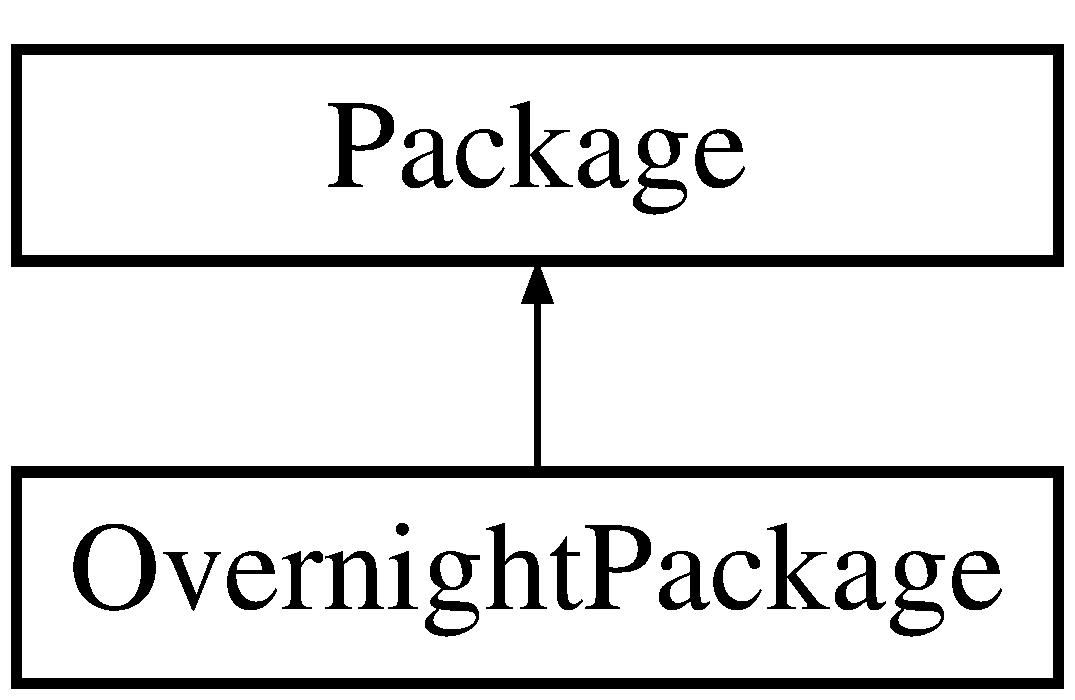
\includegraphics[height=2.000000cm]{class_overnight_package}
\end{center}
\end{figure}
\subsection*{Public Member Functions}
\begin{DoxyCompactItemize}
\item 
\mbox{\Hypertarget{class_overnight_package_a14662a2815eeafe4f7b38d74405eddd1}\label{class_overnight_package_a14662a2815eeafe4f7b38d74405eddd1}} 
{\bfseries Overnight\+Package} (string sender\+\_\+n, string sender\+\_\+addr, string sender\+\_\+c, string sender\+\_\+s, string sender\+\_\+Z, string recipient\+\_\+n, string recipient\+\_\+addr, string recipient\+\_\+c, string recipient\+\_\+s, string recipient\+\_\+Z, double wei, double cost, double delivery\+\_\+fee)
\item 
\mbox{\Hypertarget{class_overnight_package_a5c9b4980a9801f36fe4e3174af867f89}\label{class_overnight_package_a5c9b4980a9801f36fe4e3174af867f89}} 
double \mbox{\hyperlink{class_overnight_package_a5c9b4980a9801f36fe4e3174af867f89}{calculate\+Cost}} ()
\begin{DoxyCompactList}\small\item\em Calculating Cost for \mbox{\hyperlink{class_overnight_package}{Overnight\+Package}}. \end{DoxyCompactList}\item 
\mbox{\Hypertarget{class_overnight_package_a17c6d1e7b24ab8b7709f4d71ae2655db}\label{class_overnight_package_a17c6d1e7b24ab8b7709f4d71ae2655db}} 
double {\bfseries getovernight\+\_\+delivery\+\_\+fee} ()
\item 
\mbox{\Hypertarget{class_overnight_package_a16eacae64803942b64c638ccf5d0616a}\label{class_overnight_package_a16eacae64803942b64c638ccf5d0616a}} 
void {\bfseries setovernight\+\_\+delivery\+\_\+fee} (double delivery\+\_\+fee)
\end{DoxyCompactItemize}


The documentation for this class was generated from the following files\+:\begin{DoxyCompactItemize}
\item 
Overnight\+Package.\+h\item 
Overnight\+Package.\+cpp\end{DoxyCompactItemize}

\hypertarget{class_package}{}\section{Package Class Reference}
\label{class_package}\index{Package@{Package}}
Inheritance diagram for Package\+:\begin{figure}[H]
\begin{center}
\leavevmode
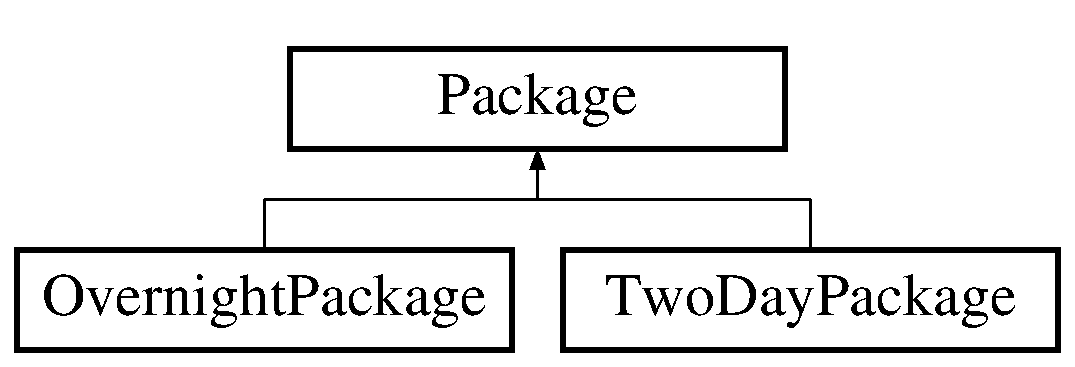
\includegraphics[height=2.000000cm]{class_package}
\end{center}
\end{figure}
\subsection*{Public Member Functions}
\begin{DoxyCompactItemize}
\item 
\mbox{\hyperlink{class_package_a3b3ccbce09176e6c7acb16906bfe0fce}{Package}} (string sender\+\_\+n, string sender\+\_\+addr, string sender\+\_\+c, string sender\+\_\+s, string sender\+\_\+Z, string recipient\+\_\+n, string recipient\+\_\+addr, string recipient\+\_\+c, string recipient\+\_\+s, string recipient\+\_\+Z, double wei, double cost)
\begin{DoxyCompactList}\small\item\em Constructor. \end{DoxyCompactList}\item 
\mbox{\Hypertarget{class_package_ace5577424f5b709217608398dc31996a}\label{class_package_ace5577424f5b709217608398dc31996a}} 
void \mbox{\hyperlink{class_package_ace5577424f5b709217608398dc31996a}{setsender\+\_\+name}} (string sender\+\_\+n)
\begin{DoxyCompactList}\small\item\em Set and Get Functions. \end{DoxyCompactList}\item 
\mbox{\Hypertarget{class_package_aeb55d6547f28f2a4577ebf0be55b816a}\label{class_package_aeb55d6547f28f2a4577ebf0be55b816a}} 
string {\bfseries getsender\+\_\+name} ()
\item 
\mbox{\Hypertarget{class_package_a6bb1b20a876a8212a2bf8ff998d866a9}\label{class_package_a6bb1b20a876a8212a2bf8ff998d866a9}} 
void {\bfseries setsender\+\_\+address} (string sender\+\_\+addr)
\item 
\mbox{\Hypertarget{class_package_adf5ce398435f90bec468d87e31fe1d6a}\label{class_package_adf5ce398435f90bec468d87e31fe1d6a}} 
string {\bfseries getsender\+\_\+address} ()
\item 
\mbox{\Hypertarget{class_package_a6f0b8f51e6d72bfa3c5b2d9579b3dc3f}\label{class_package_a6f0b8f51e6d72bfa3c5b2d9579b3dc3f}} 
void {\bfseries setsender\+\_\+city} (string sender\+\_\+c)
\item 
\mbox{\Hypertarget{class_package_a539fc1afbd3c07c1347974d1e90a323c}\label{class_package_a539fc1afbd3c07c1347974d1e90a323c}} 
string {\bfseries get\+Send\+City} ()
\item 
\mbox{\Hypertarget{class_package_a63208941e737271d156e8489c298d6cc}\label{class_package_a63208941e737271d156e8489c298d6cc}} 
void {\bfseries setsender\+\_\+state} (string sender\+\_\+s)
\item 
\mbox{\Hypertarget{class_package_a09627c4b99dfb508a92c884f4f7547b7}\label{class_package_a09627c4b99dfb508a92c884f4f7547b7}} 
string {\bfseries getsender\+\_\+state} ()
\item 
\mbox{\Hypertarget{class_package_a56cf09ba2ac0d10ccf1661d9394c6b85}\label{class_package_a56cf09ba2ac0d10ccf1661d9394c6b85}} 
void {\bfseries setsender\+\_\+\+Z\+IP} (string sender\+\_\+Z)
\item 
\mbox{\Hypertarget{class_package_a66539199f86eed481721ff0851676109}\label{class_package_a66539199f86eed481721ff0851676109}} 
string {\bfseries getsender\+\_\+\+Z\+IP} ()
\item 
\mbox{\Hypertarget{class_package_a7f22cd63211c0c766ddf32926362c885}\label{class_package_a7f22cd63211c0c766ddf32926362c885}} 
void {\bfseries setrecipient\+\_\+name} (string recipient\+\_\+n)
\item 
\mbox{\Hypertarget{class_package_a8022d4210f41bc9e0dae744aae7c5bbc}\label{class_package_a8022d4210f41bc9e0dae744aae7c5bbc}} 
string {\bfseries getrecipient\+\_\+name} ()
\item 
\mbox{\Hypertarget{class_package_a5ec7ebc5d7640f5f8c8e1747689b5e8a}\label{class_package_a5ec7ebc5d7640f5f8c8e1747689b5e8a}} 
void {\bfseries setrecipient\+\_\+address} (string recipient\+\_\+addr)
\item 
\mbox{\Hypertarget{class_package_a68e6c329e3ee89e578befa648b3e47e8}\label{class_package_a68e6c329e3ee89e578befa648b3e47e8}} 
string {\bfseries getrecipient\+\_\+address} ()
\item 
\mbox{\Hypertarget{class_package_a6a9facae5d8ccf6a6cd5128a8b3583e2}\label{class_package_a6a9facae5d8ccf6a6cd5128a8b3583e2}} 
void {\bfseries setrecipient\+\_\+city} (string recipient\+\_\+c)
\item 
\mbox{\Hypertarget{class_package_aa9afd5572cd63edc9d5b754641e6ca4f}\label{class_package_aa9afd5572cd63edc9d5b754641e6ca4f}} 
string {\bfseries getrecipient\+\_\+city} ()
\item 
\mbox{\Hypertarget{class_package_a94160244d96deaeb9361e544e98d0a9f}\label{class_package_a94160244d96deaeb9361e544e98d0a9f}} 
void {\bfseries setrecipient\+\_\+state} (string recipient\+\_\+s)
\item 
\mbox{\Hypertarget{class_package_a355178fb4b38c4b11620b96e67f9bc1c}\label{class_package_a355178fb4b38c4b11620b96e67f9bc1c}} 
string {\bfseries getrecipient\+\_\+state} ()
\item 
\mbox{\Hypertarget{class_package_a9ae0894bf750037e3923b1d9d410246c}\label{class_package_a9ae0894bf750037e3923b1d9d410246c}} 
void {\bfseries setrecipient\+\_\+\+Z\+IP} (string recipient\+\_\+Z)
\item 
\mbox{\Hypertarget{class_package_a6943b57b109b1c185aab93e6c0ad8c1d}\label{class_package_a6943b57b109b1c185aab93e6c0ad8c1d}} 
string {\bfseries getrecipient\+\_\+\+Z\+IP} ()
\item 
\mbox{\Hypertarget{class_package_a2734b7fd507a259f34b6ae7a42044cc5}\label{class_package_a2734b7fd507a259f34b6ae7a42044cc5}} 
void {\bfseries setweight} (double w)
\item 
\mbox{\Hypertarget{class_package_a794c750fbdc0a0bbf051ef84ff155256}\label{class_package_a794c750fbdc0a0bbf051ef84ff155256}} 
double {\bfseries getweight} ()
\item 
\mbox{\Hypertarget{class_package_acce59769e49209f03205a21057bb27c0}\label{class_package_acce59769e49209f03205a21057bb27c0}} 
void {\bfseries setcostperounce} (double cost)
\item 
\mbox{\Hypertarget{class_package_a8b292251f4b91f04ec7752a0f4bf253c}\label{class_package_a8b292251f4b91f04ec7752a0f4bf253c}} 
double {\bfseries getcostperounce} ()
\item 
\mbox{\Hypertarget{class_package_a39e17c4cb7f41b9e4501d1a88a57e862}\label{class_package_a39e17c4cb7f41b9e4501d1a88a57e862}} 
double \mbox{\hyperlink{class_package_a39e17c4cb7f41b9e4501d1a88a57e862}{calculate\+Cost}} ()
\begin{DoxyCompactList}\small\item\em Calculating Cost. \end{DoxyCompactList}\end{DoxyCompactItemize}


\subsection{Constructor \& Destructor Documentation}
\mbox{\Hypertarget{class_package_a3b3ccbce09176e6c7acb16906bfe0fce}\label{class_package_a3b3ccbce09176e6c7acb16906bfe0fce}} 
\index{Package@{Package}!Package@{Package}}
\index{Package@{Package}!Package@{Package}}
\subsubsection{\texorpdfstring{Package()}{Package()}}
{\footnotesize\ttfamily Package\+::\+Package (\begin{DoxyParamCaption}\item[{string}]{sender\+\_\+n,  }\item[{string}]{sender\+\_\+addr,  }\item[{string}]{sender\+\_\+c,  }\item[{string}]{sender\+\_\+s,  }\item[{string}]{sender\+\_\+Z,  }\item[{string}]{recipient\+\_\+n,  }\item[{string}]{recipient\+\_\+addr,  }\item[{string}]{recipient\+\_\+c,  }\item[{string}]{recipient\+\_\+s,  }\item[{string}]{recipient\+\_\+Z,  }\item[{double}]{wei,  }\item[{double}]{cost }\end{DoxyParamCaption})}



Constructor. 

Checking whether Weight and Cost are positive 

The documentation for this class was generated from the following files\+:\begin{DoxyCompactItemize}
\item 
Package.\+h\item 
Package.\+cpp\end{DoxyCompactItemize}

\hypertarget{class_two_day_package}{}\section{Two\+Day\+Package Class Reference}
\label{class_two_day_package}\index{Two\+Day\+Package@{Two\+Day\+Package}}
Inheritance diagram for Two\+Day\+Package\+:\begin{figure}[H]
\begin{center}
\leavevmode
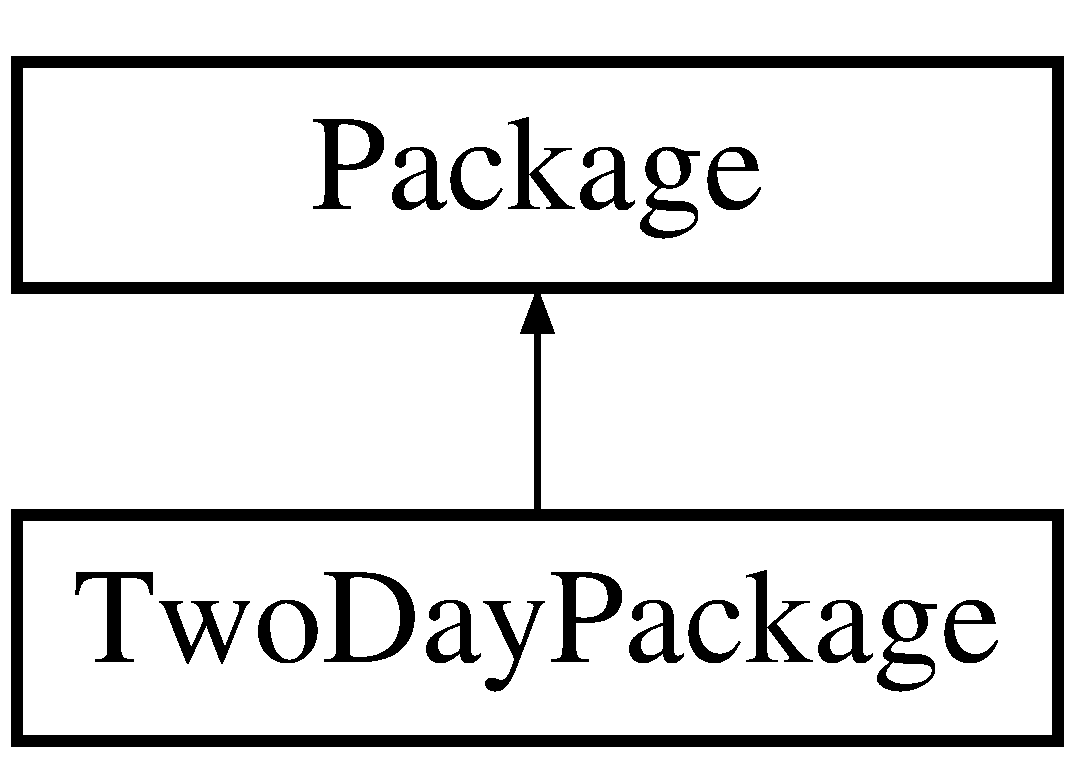
\includegraphics[height=2.000000cm]{class_two_day_package}
\end{center}
\end{figure}
\subsection*{Public Member Functions}
\begin{DoxyCompactItemize}
\item 
\mbox{\Hypertarget{class_two_day_package_a95838cf123fb1e9706a957cf049c5e25}\label{class_two_day_package_a95838cf123fb1e9706a957cf049c5e25}} 
{\bfseries Two\+Day\+Package} (string sender\+\_\+n, string sender\+\_\+addr, string sender\+\_\+c, string sender\+\_\+s, string sender\+\_\+Z, string recipient\+\_\+n, string recipient\+\_\+addr, string recipient\+\_\+c, string recipient\+\_\+s, string recipient\+\_\+Z, double wei, double cost, double delivery\+\_\+fee)
\item 
\mbox{\Hypertarget{class_two_day_package_a8f794e7e88e802b0b7089174e430cd96}\label{class_two_day_package_a8f794e7e88e802b0b7089174e430cd96}} 
double {\bfseries gettwo\+\_\+day\+\_\+delivery\+\_\+fee} ()
\item 
\mbox{\Hypertarget{class_two_day_package_a6c5cb416afb7558e1eb2a6a709d44ead}\label{class_two_day_package_a6c5cb416afb7558e1eb2a6a709d44ead}} 
void {\bfseries settwo\+\_\+day\+\_\+delivery\+\_\+fee} (double delivery\+\_\+fee)
\item 
\mbox{\Hypertarget{class_two_day_package_ac87bb9d651b859d1049a003b6659037c}\label{class_two_day_package_ac87bb9d651b859d1049a003b6659037c}} 
double \mbox{\hyperlink{class_two_day_package_ac87bb9d651b859d1049a003b6659037c}{calculate\+Cost}} ()
\begin{DoxyCompactList}\small\item\em Calculating Cost for \mbox{\hyperlink{class_two_day_package}{Two\+Day\+Package}}. \end{DoxyCompactList}\end{DoxyCompactItemize}


The documentation for this class was generated from the following files\+:\begin{DoxyCompactItemize}
\item 
Two\+Day\+Package.\+h\item 
Two\+Day\+Package.\+cpp\end{DoxyCompactItemize}

%--- End generated contents ---

% Index
\backmatter
\newpage
\phantomsection
\clearemptydoublepage
\addcontentsline{toc}{chapter}{Index}
\printindex

\end{document}
